\section{Description}
This module is responsible for storing users and patterns, communicating with
the client and running the Siddhi engine. Furthermore, it is the endpoint where
all sensors have to sent their data in order to be processed by the Siddhi engine.
The server primarily consists of
\begin{itemize}
    \item controllers - to manage the stored data
    \item handlers - to coordinate network communication
    \item the Siddhi engine - to process events and detect patterns
    \item loggers - to keep a log of all events, errors and actions occuring
    \item command-line-interface (cli) - to provide the admin console
\end{itemize}

\section{Overview}
\FloatBarrier
\begin{figure}
    \centering
    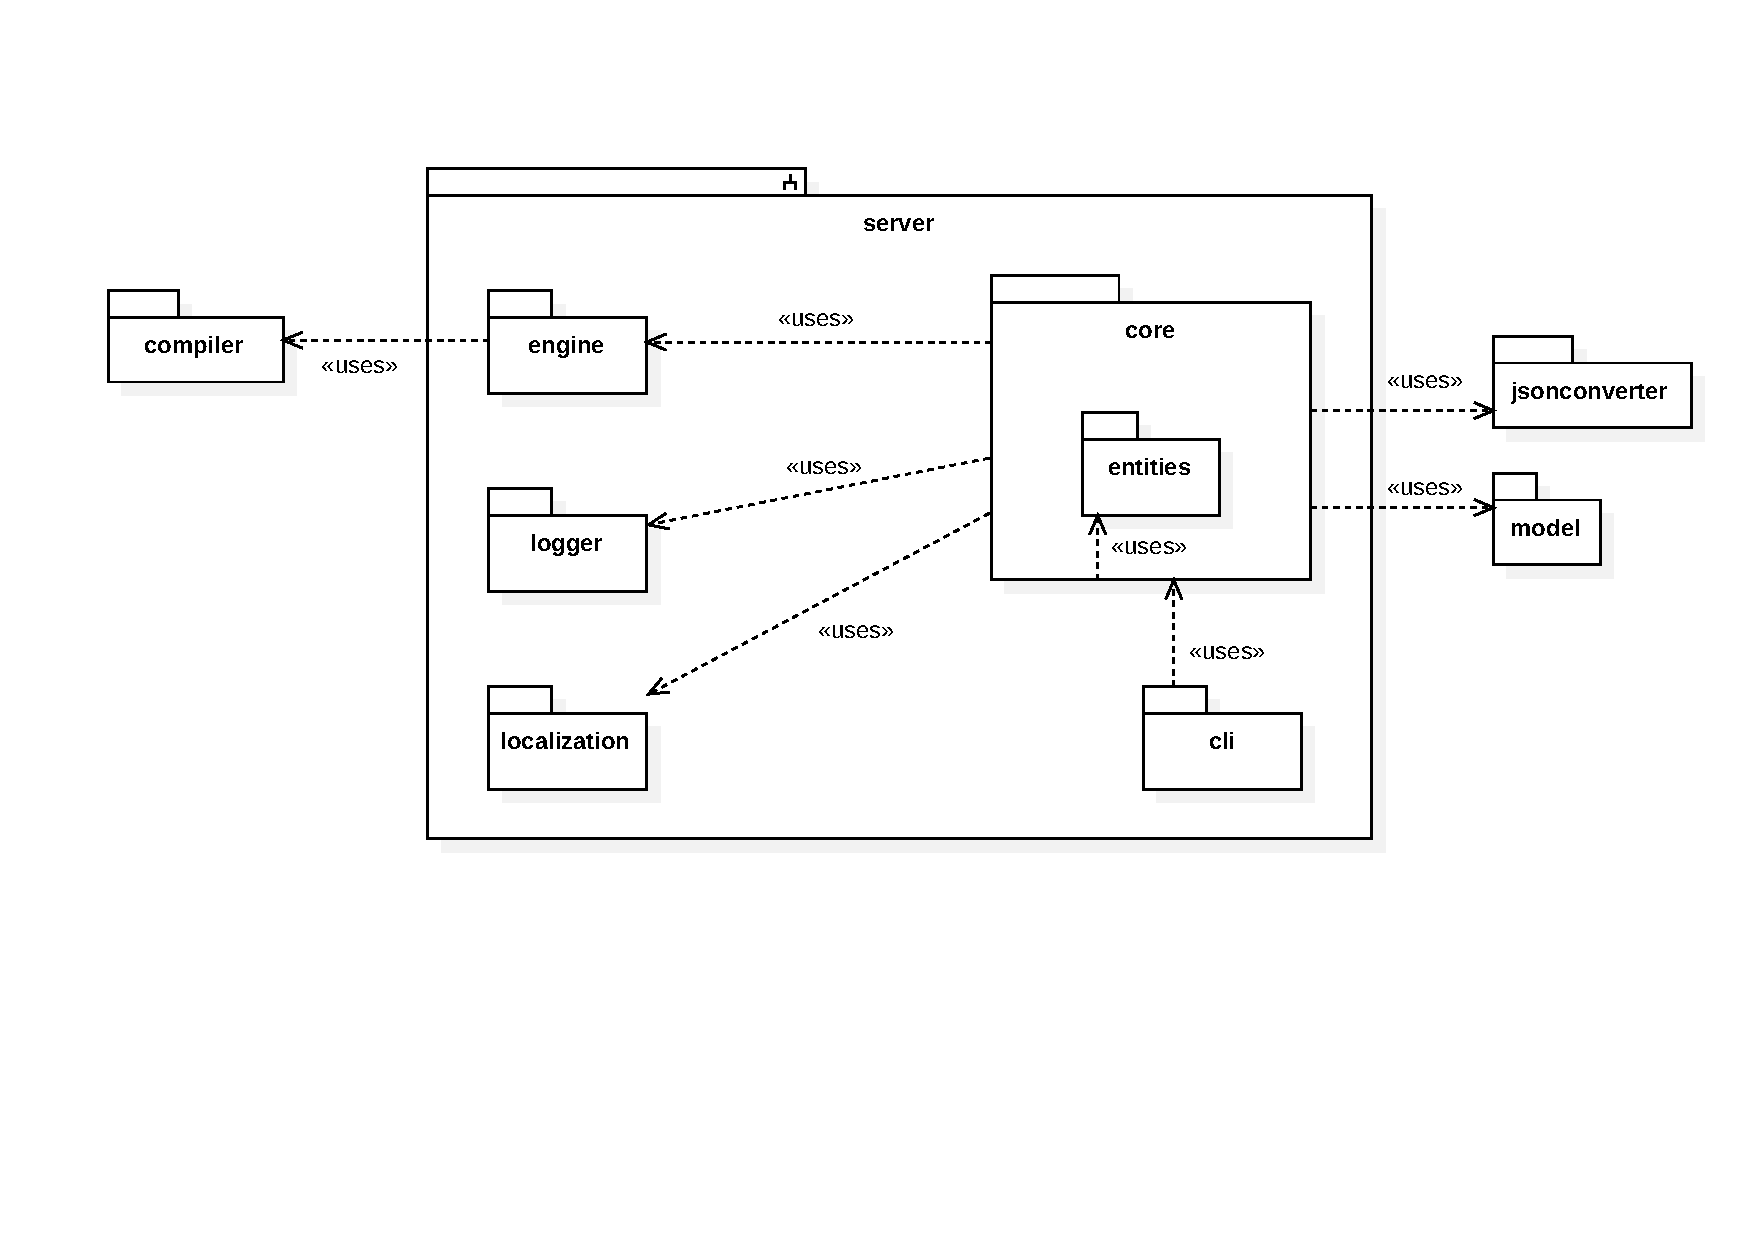
\includegraphics[width=\textwidth]{../module_res/server-package.pdf}
    \caption{UML package Diagram of the server module with uses-relations.
    (Uses-relations between other modules were omitted).
    \label{fig:server-package}}
\end{figure}
\FloatBarrier


\section{Sequence Diagrams}
The following UML sequence diagrams specify the communication between classes
within this module for typcial use cases like
\enquote{Add new user} (\autoref{fig:server-sd-addusercmd}),
\enquote{Deploy pattern} (\autoref{fig:server-sd-deploypatternroute}) and
\enquote{Receive event from sensor} (\autoref{fig:server-sd-sendevent}).
\emph{(Notice: Logging operations were omitted for clarity).}

\FloatBarrier

\begin{figure}[h]
    \centering
    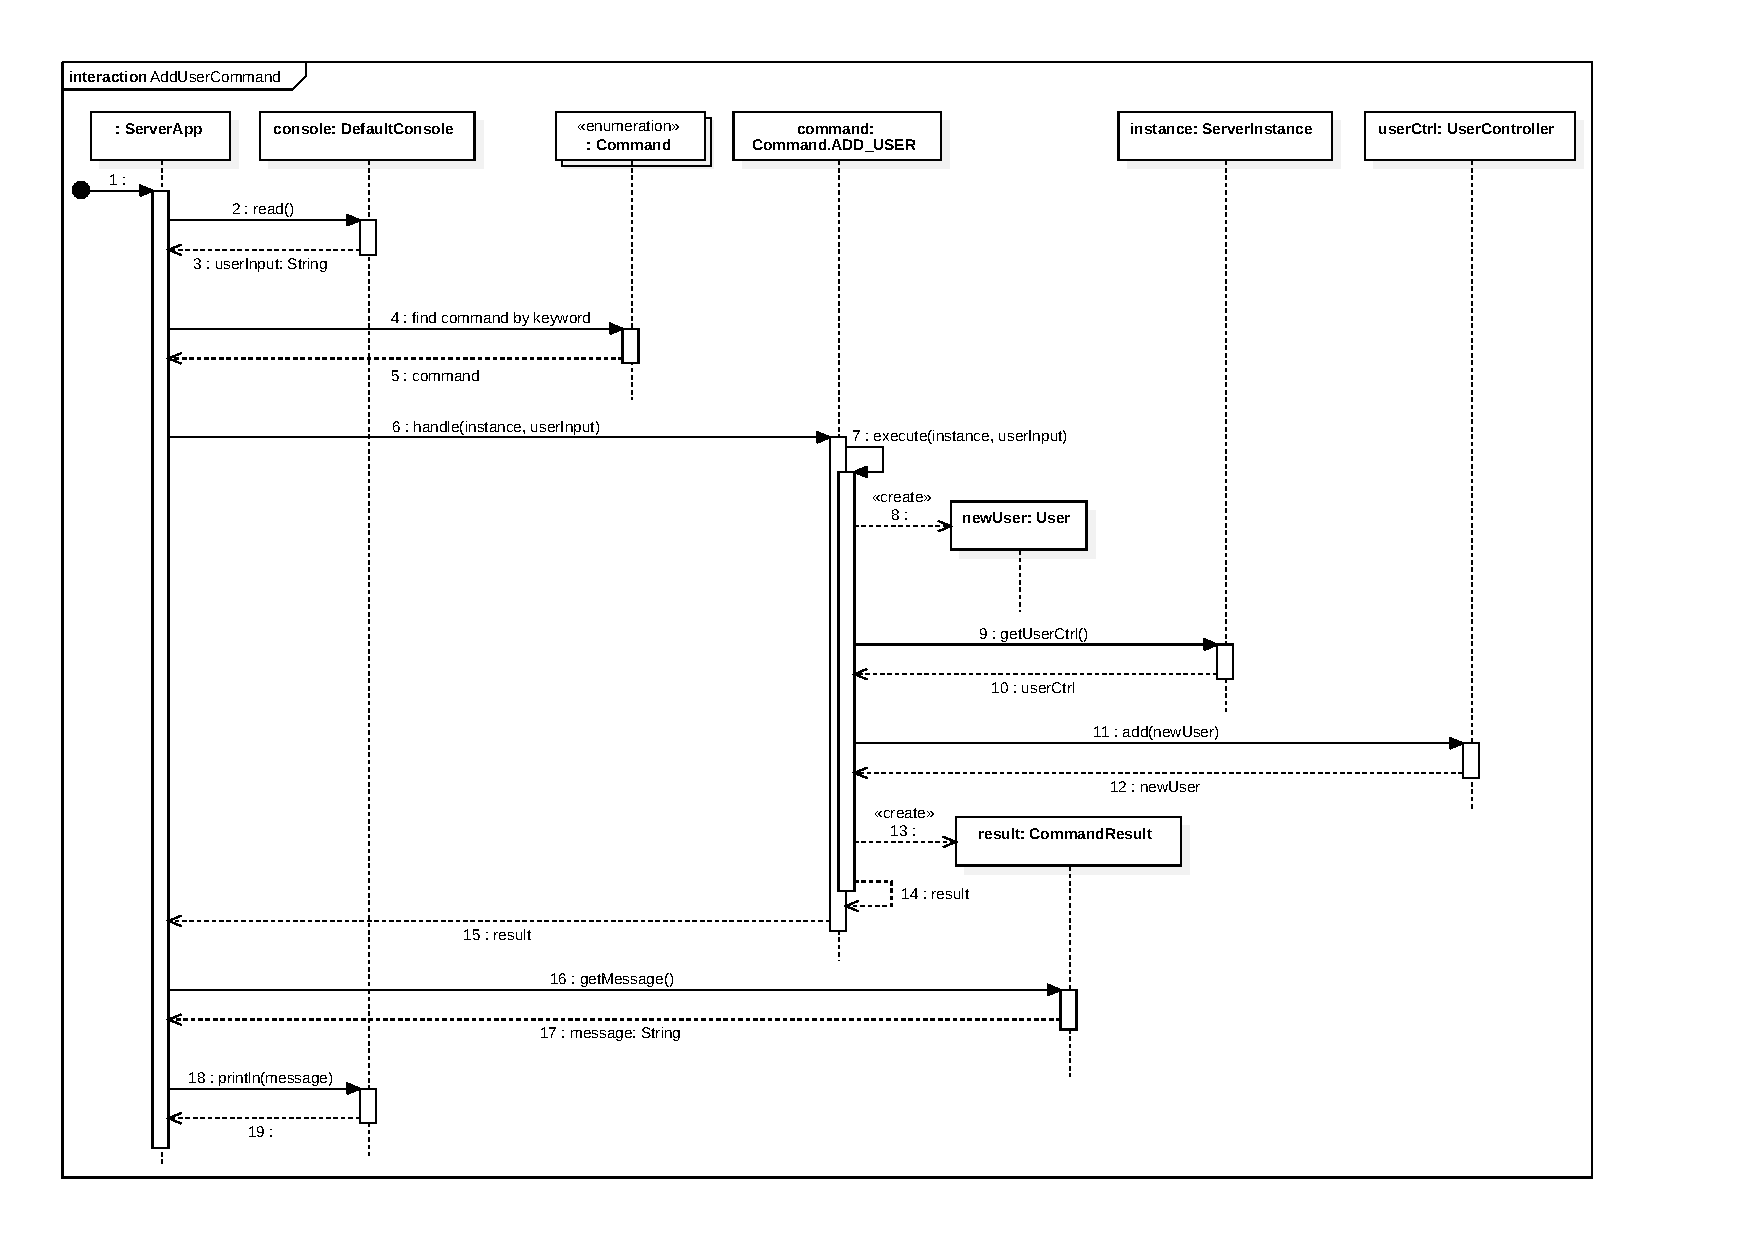
\includegraphics[width=\textwidth]{../module_res/server-sd-addusercmd.pdf}
    \caption{Sequence Diagram:
        An admin adds a new user by executing the corresponding command in the
        admin console.
    \label{fig:server-sd-addusercmd}}
\end{figure}

\begin{figure}[h]
    \centering
    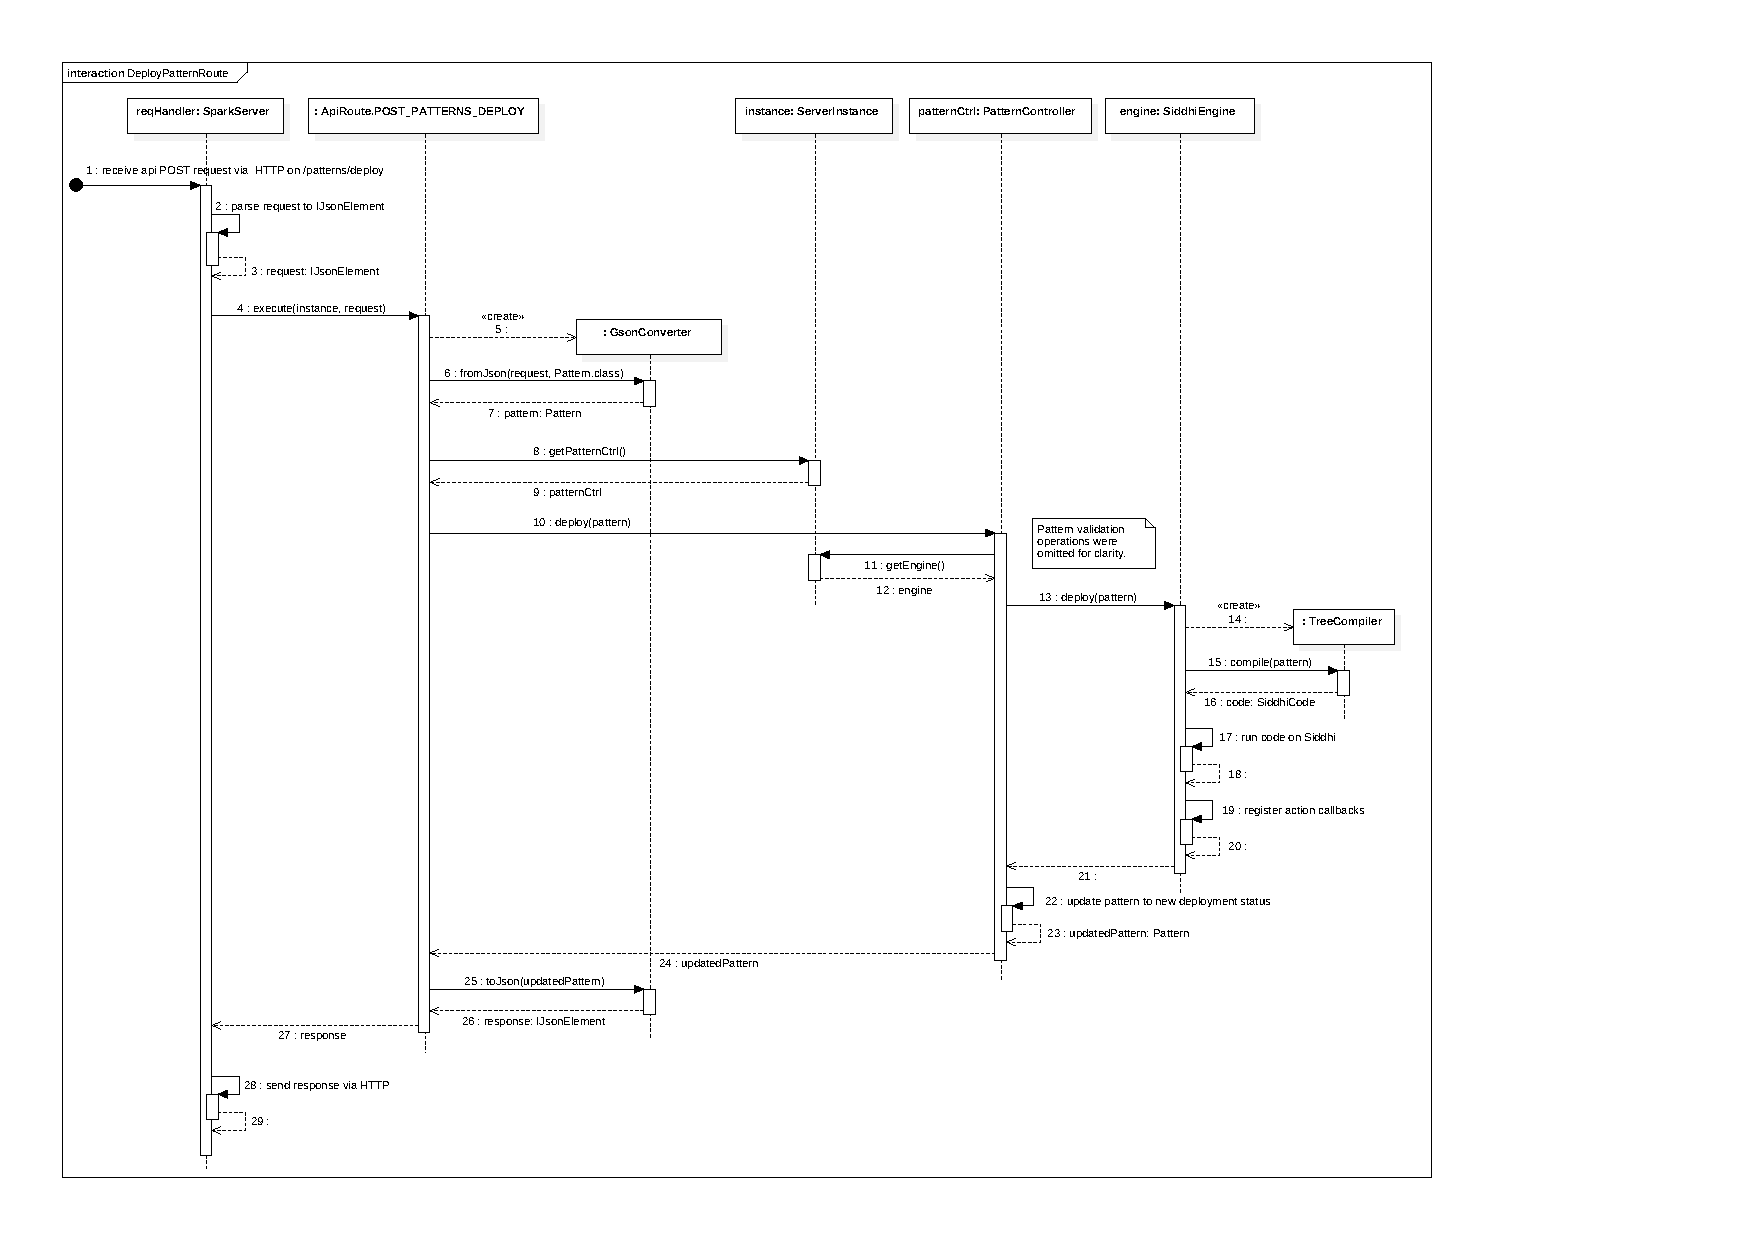
\includegraphics[width=\textwidth]{../module_res/server-sd-deploypatternroute.pdf}
    \caption{Sequence Diagram:
        The server receives an request (e.g. from a client) to deploy a pattern
        to the Siddhi engine.
    \label{fig:server-sd-deploypatternroute}}
\end{figure}

\begin{figure}[h]
    \centering
    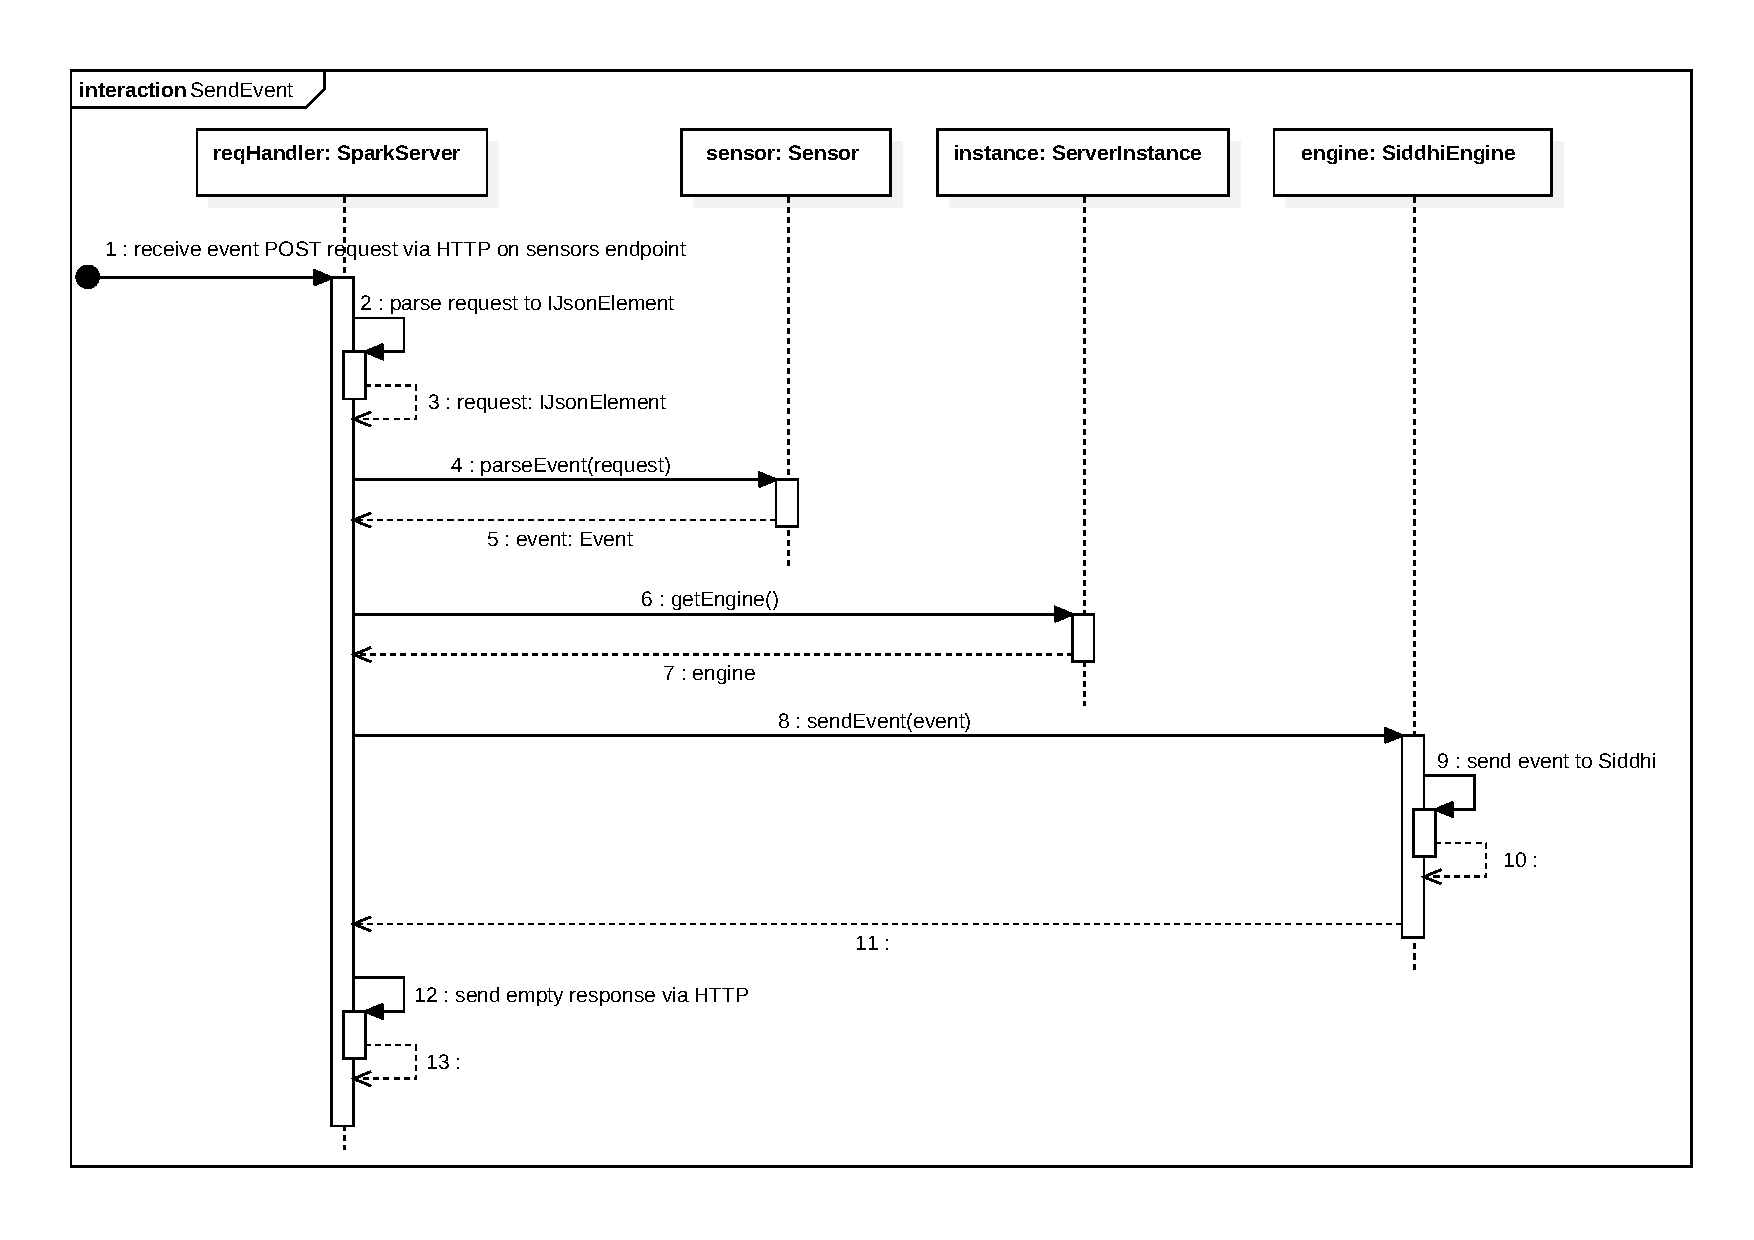
\includegraphics[width=\textwidth]{../module_res/server-sd-sendevent.pdf}
    \caption{Sequence Diagram: 
    \label{fig:server-sd-sendevent}}
\end{figure}

\FloatBarrier
